\documentclass[a4paper,12pt]{report}
\usepackage{graphicx}
\graphicspath{{picaa/}}
\usepackage{listings}
\usepackage{amsmath}
\usepackage[T2A]{fontenc}
\usepackage[utf8]{inputenc}
\usepackage[english,russian]{babel}
\usepackage{pgfplots} 
\usepackage{indentfirst}
\parindent=1cm

\usepackage{geometry}
\geometry{left=2cm}
\geometry{right=1.5cm}
\geometry{top=1cm}
\geometry{bottom=2cm}
\lstset{language = Python,
keywordstyle = \color{orange},
stringstyle = \color{green},
commentstyle = \color{red},
columns = fullflexible,
captionpos = t
}

\begin{document}

    \begin{titlepage}

        \begin{center}
            \large
            \textbf{Государственное образовательное учреждение высшего профессионального образования\\
            “Московский государственный технический университет имени Н.Э.Баумана”\\}
            
\includegraphics{bmstu-logo.png}
			\vspace{1cm}
            
            \textsc{Дисциплина: Анализ алгоритмов}
            \vspace{0.5cm}
                
            \textsc{Лабораторная работа №1}
            \vspace{1cm}
            
            {\LARGE \textbf{Расстояние Левенштейна}}
            \vspace{3cm}
                    
            \begin{flushright}
            	Студент группы ИУ7-55Б,\\   
            	Руднев К. К.,\\
            	\vspace{0.5cm}
            	Преподаватель,\\
            	Волкова Л. Л.,\\
            	Строганов Ю. В.
            	
            \end{flushright}
            \vfill
            
            2019 г.
            
            \end{center}

    \end{titlepage}

	\setcounter{page}{2}
	
    \begin{center}
        \textbf{Введение\\}
        \begin{flushleft}
			Цель работы: изучение метода динамического программирования на материале алгоритмов Левенштейна и Дамерау-Левенштейна.\\
			Задачи работы:\\
			\begin{enumerate} 
				\item изучение алгоритмов Левенштейна и Дамерау-Левенштейна нахождения расстояния между строками;\\
				\item применение метода динамического программирования для матричной реализации указанных алгоритмов;\\
				\item получение практических навыков реализации указанных алгоритмов: двух алгоритмов в матричной версии и одного из алгоритмов в рекурсивной версии;\\
				\item сравнительный анализ линейной и рекурсивной реализаций выбранного алгоритма определения расстояния между строками по затрачиваемым ресурсам (времени и памяти);\\
				\item экспериментальное подтверждение различий во временнóй эффективности рекурсивной и нерекурсивной реализаций выбранного алгоритма определения расстояния между строками при помощи разработанного программного обеспечения на материале замеров процессорного времени выполнения реализации на варьирующихся длинах строк;\\
				\item описание и обоснование полученных результатов в отчете о выполненной лабораторной работе, выполненного как расчётно-пояснительная записка к работе.\\
			\end{enumerate}
        \end{flushleft}
        \label{sec:intro}
    \end{center}

    \newpage

    \begin{center}
        \textbf{1 Аналитическая часть}
        \label{sec:analitic_part}
        \begin{flushleft}
        	В рамках раздела будет дано аналитическое описание алгоритмов Левенштейна и Дамерау-Левенштейна.
        \end{flushleft}

        \textbf{1.1 Описание алгоритмов\\}
        \vspace{0,5cm}
        
        \begin{flushleft}
	        Расстояние Левенштейна (также известно как редакционное расстояние) между двумя строками есть минимальное число операций удаления, вставки, замены символа строки для преобразования одной строки к другой. Для решения поставленной задачи существует несколько возможных алгоритмов. Среди них алгоритмы Левенштейна и Дамерау-Левенштейна.\\
	       	\vspace{0,5cm}
	        Допустим, имеются две строки S1 и S2, их длины соответсвенно равны M и N. Тогда для для нахождения расстояния Левенштейна можно воспользоваться следующей формулой:\\
        	
	        \[
	        D(i,j)=\begin{cases}
	        max(i,j)\ if\ min(i,j) == 0\\
	        min\begin{cases}
	        D(i,j-1) + 1\\
	        D(i-1,j) + 1\\
	        D(i-1,j-1) + (S1[i] <> S2[j])
	        \end{cases}
	        \end{cases}
	        \]
	    
		    	Для нахождения расстояния Дамерау-Левенштейна можно воспользоваться следующей формулой:\\
		    	
		    	\[
		    	D(i,j)=\begin{cases}
		    	max(i,j)\ if\ min(i,j) == 0\\
		    	min\begin{cases}
		    	D(i,j-1) + 1\\
		    	D(i-1,j) + 1\\
		    	D(i-1,j-1) + (S1[i] <> S2[j])\\
		    	D(i-2,j-2) + 1
		    	\end{cases} \ if \ i,j>1 \ and \ Transpose\\
		    	min\begin{cases}
		    	D(i,j-1) + 1\\
		    	D(i-1,j) + 1\\
		    	D(i-1,j-1) + (S1[i] <> S2[j]),
		    	\end{cases}
		    	\end{cases}
		    	\]
		    	\[ \texttt{где} \ Transpose = S1[i] == S2[j-1] \ and \ S1[i-1] == S2[j] \]
	    	\end{flushleft}
    \end{center}

    \newpage

    \begin{center}
        \textbf{2 Конструкторская часть}
        \label{sec:construct_part}
		\begin{flushleft}
			В дальнейшем на рисунках \ref{ris:recLevD1}-\ref{ris:matLev3}  будут представлены схемы расматриваемых алгоритмов.
			Рисунки \ref{ris:recLevD1}-\ref{ris:recLevD2} изображают схему рекурсивного алгоритма нахождения расстояния Дамерау-Левенштейна.
			Рисунки \ref{ris:matLevD1}-\ref{ris:matLevD3} изображают схему матричного алгоритма нахождения расстояния Дамерау-Левенштейна. 
			Рисунки \ref{ris:matLev1}-\ref{ris:matLev3} изображают схему матричного алгоритма нахождения расстояния Левенштейна.
		\end{flushleft}

        \textbf{2.1 Разработка алгоритмов}

		\begin{figure}[h!]
			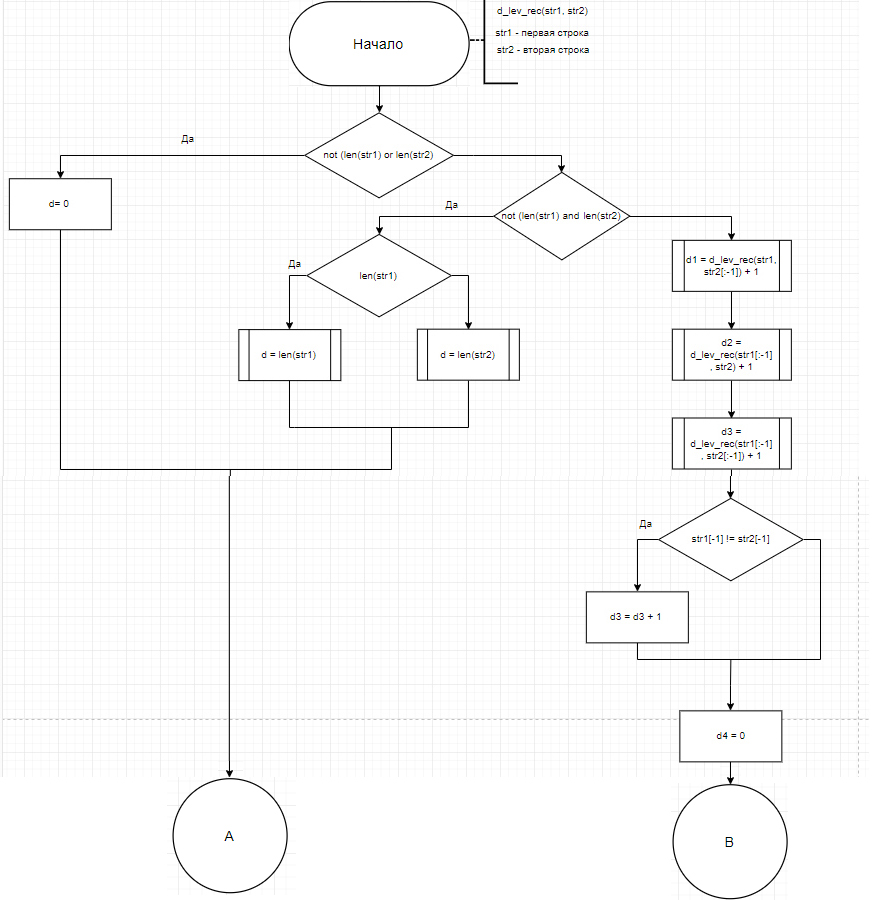
\includegraphics[width=1\linewidth]{d_lev_rec2.jpg}
			\caption{Рекурсивный алгоритм нахождения расстояния Дамерау-Левенштейна. Часть 1}
			\label{ris:recLevD1}
		\end{figure}
	
		\newpage
		\begin{figure}[h!]
			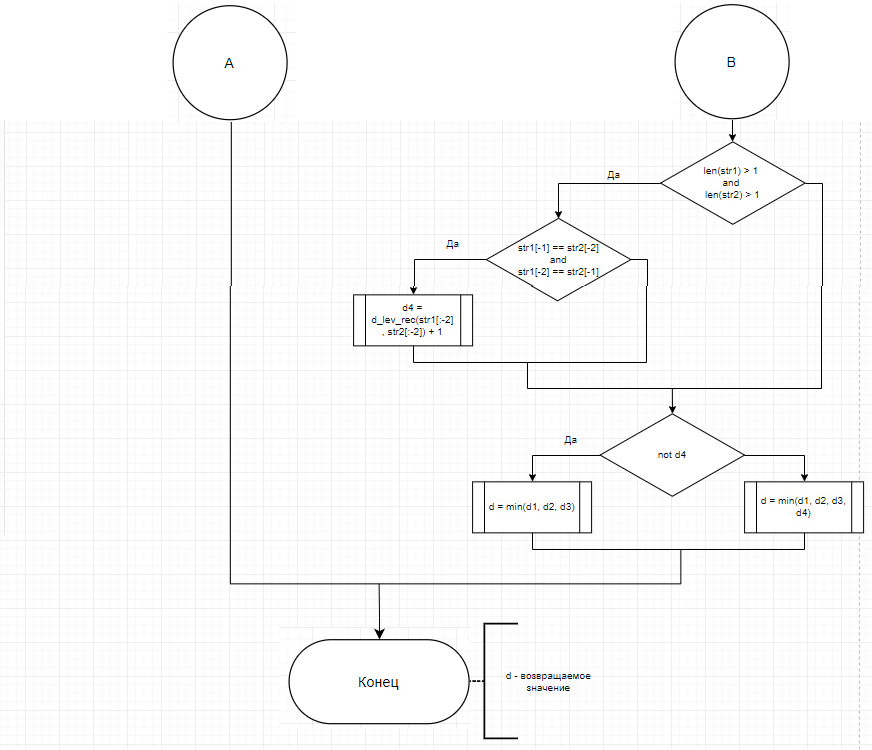
\includegraphics[width=1\linewidth]{d_lev_rec1.jpg}
			\caption{Рекурсивный алгоритм нахождения расстояния Дамерау-Левенштейна. Часть 2}
			\label{ris:recLevD2}
		\end{figure}
		
		\newpage
		\begin{figure}[h!]
			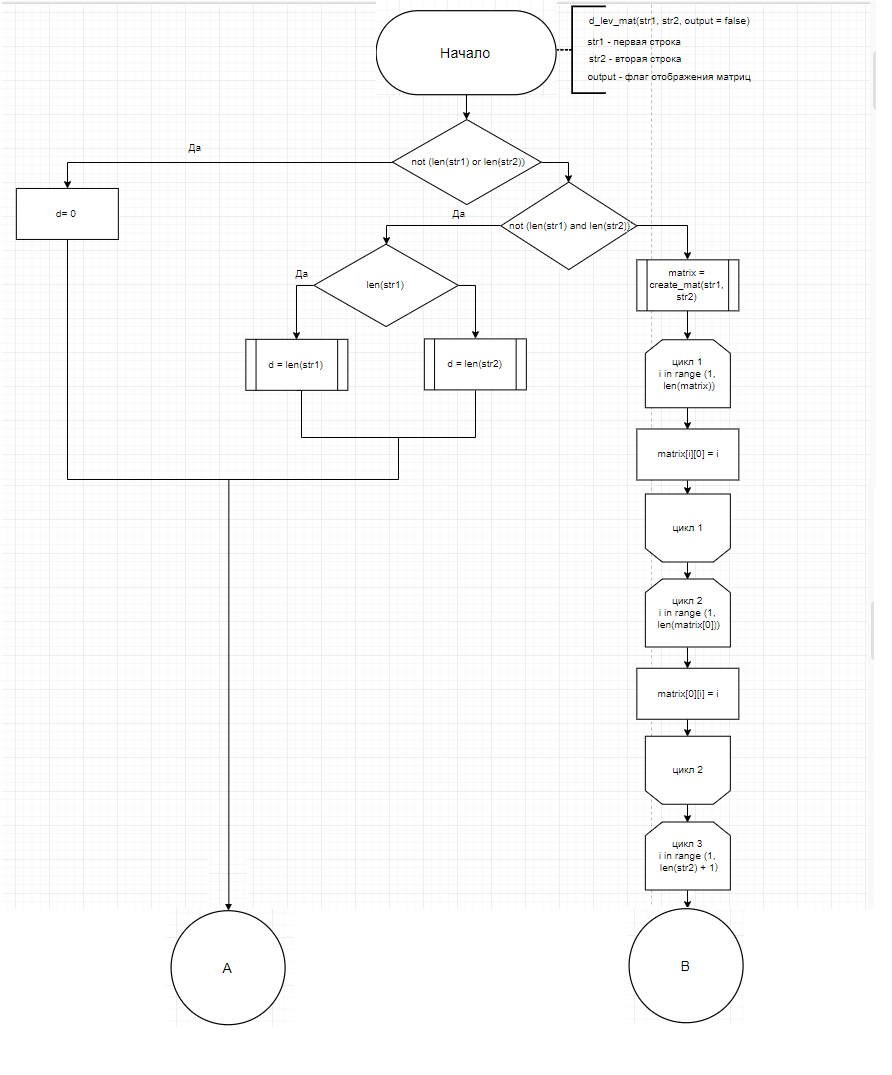
\includegraphics[width=1\linewidth]{lev_mat.jpg}
			\caption{Матричный алгоритм нахождения расстояния Дамерау-Левенштейна. Часть 1}
			\label{ris:matLevD1}
		\end{figure}
		
		\newpage
		\begin{figure}[h!]
			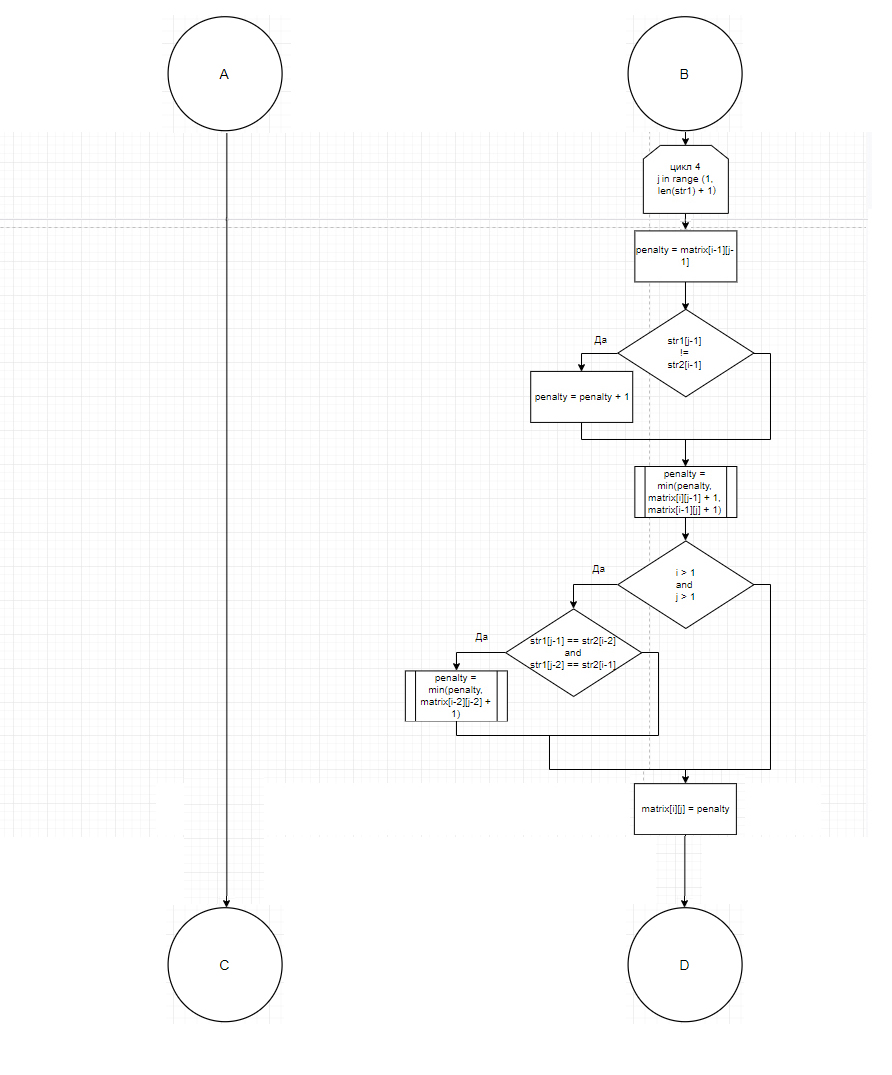
\includegraphics[width=1\linewidth]{lev_mat_end1.jpg}
			\caption{Матричный алгоритм нахождения расстояния Дамерау-Левенштейна. Часть 2}
			\label{ris:matLevD2}
		\end{figure}
		
		\newpage
		\begin{figure}[h!]
			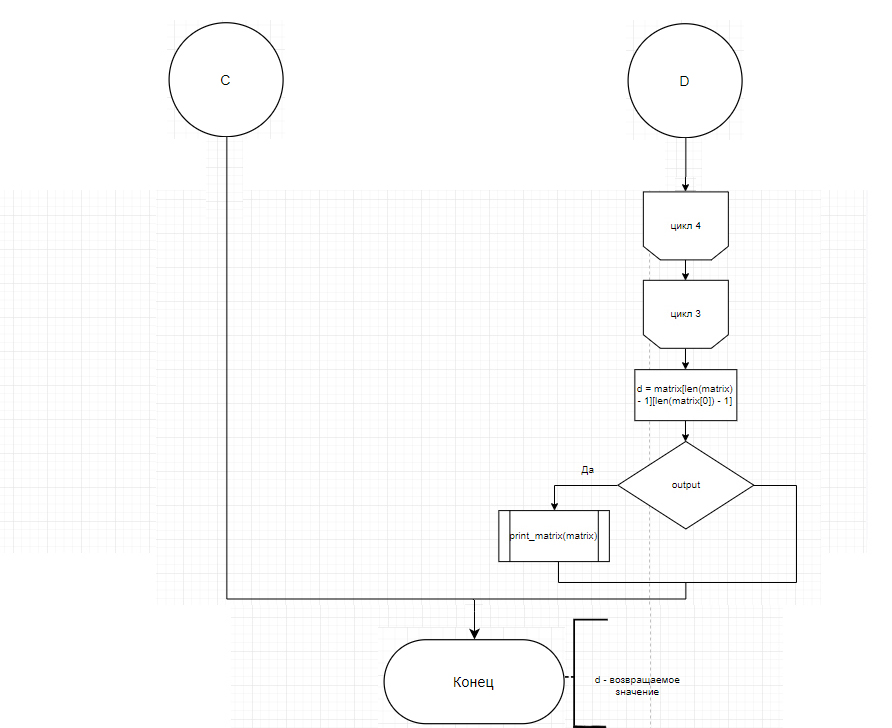
\includegraphics[width=1\linewidth]{lev_mat_end2.jpg}
			\caption{Матричный алгоритм нахождения расстояния Дамерау-Левенштейна. Часть 3}
			\label{ris:matLevD3}
		\end{figure}
		
		\newpage
		\begin{figure}[h!]
			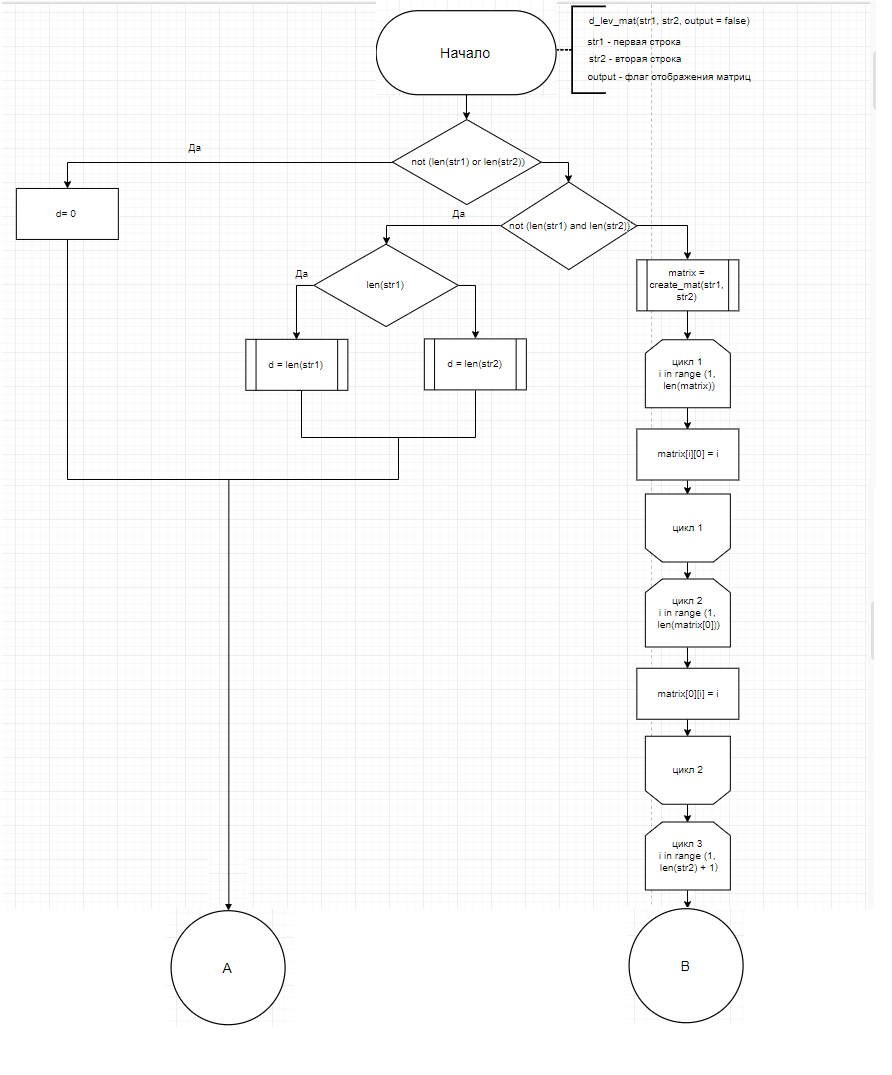
\includegraphics[width=1\linewidth]{lev_mat.jpg}
			\caption{Матричный алгоритм нахождения расстояния Левенштейна. Часть 1}
			\label{ris:matLev1}
		\end{figure}
	
		\newpage
		\begin{figure}[h!]
			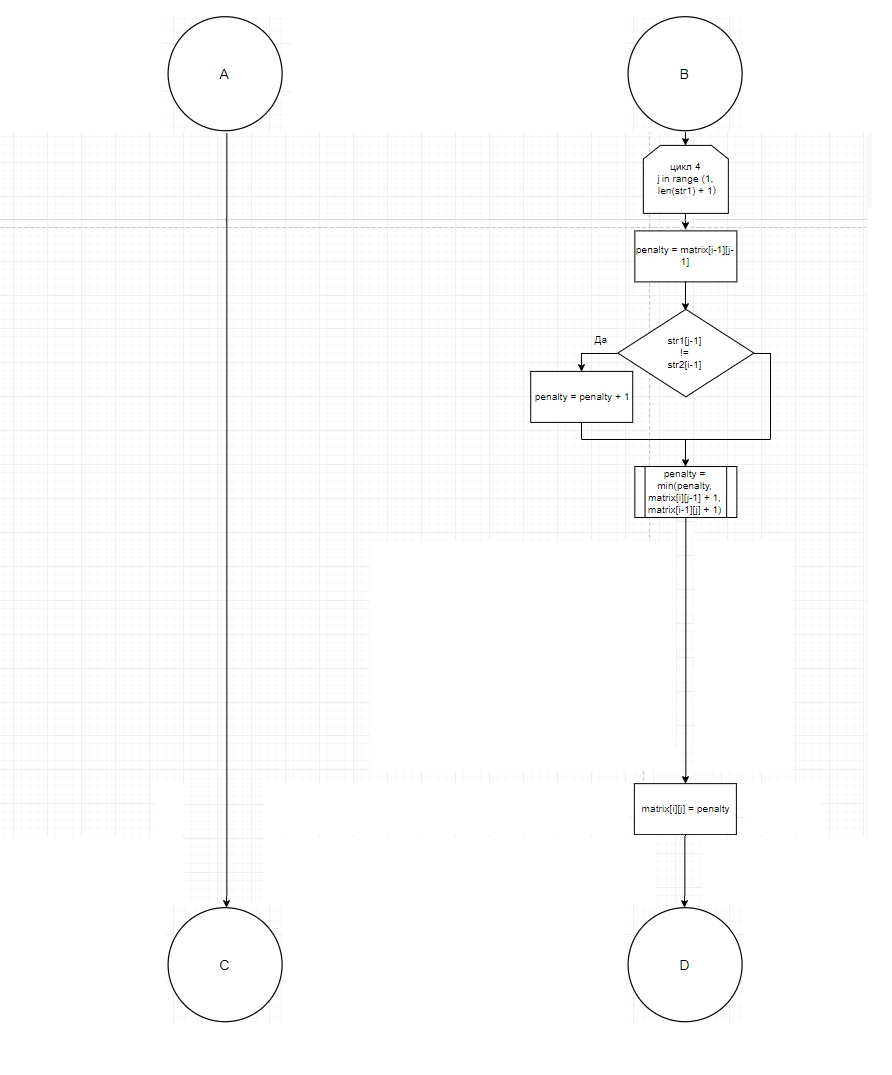
\includegraphics[width=1\linewidth]{lev_mat_end3.jpg}
			\caption{Матричный алгоритм нахождения расстояния Левенштейна. Часть 2}
			\label{ris:matLev2}
		\end{figure}
	
		\newpage
		\begin{figure}[h!]
			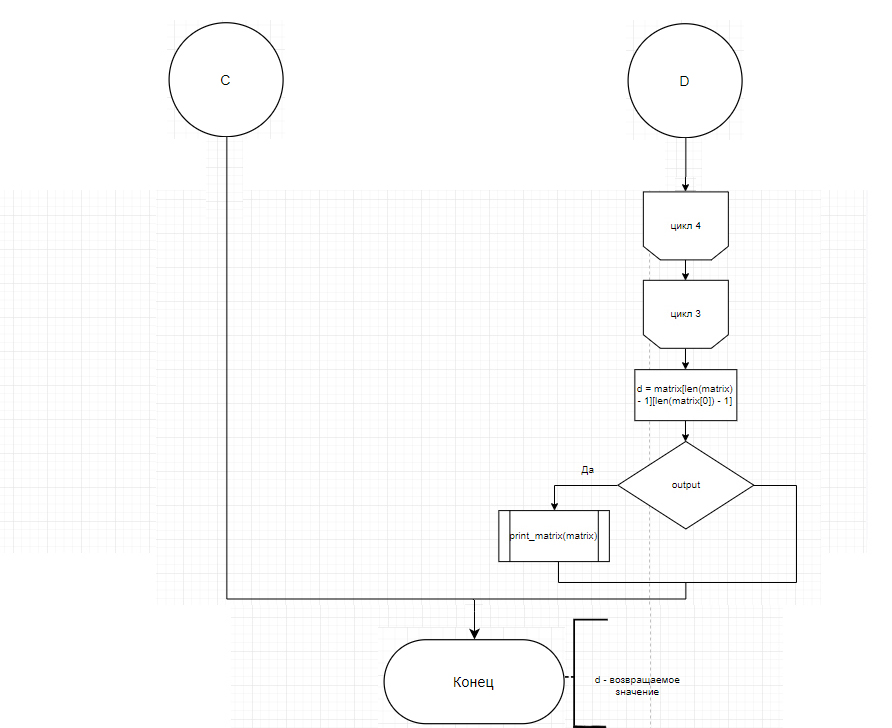
\includegraphics[width=1\linewidth]{lev_mat_end2.jpg}
			\caption{Матричный алгоритм нахождения расстояния Левенштейна. Часть 3}
			\label{ris:matLev3}
		\end{figure}
	\end{center}

    \newpage

    \begin{center}
        \textbf{3 Технологическая часть}
        \label{sec:tecnologic_part}
		\begin{flushleft}
			В рамках раздела будут описаны инструментарии разработки, выбор среды, требобования к ПО. Также будут предоставлены листинги конкретных реализаций алгоритмов.
		\end{flushleft}
	
        \textbf{3.1. Средства реализации}
        \begin{flushleft}
        	Для реализации алгоритмов использовался язык программирования Python 3.6.0 и среда разработки PyCharm Community Edition 2017.2.4 by JetBrains. У меня есть определенный опыт работы с данным языком, которого будет достаточно для реализации текущей лабораторной работы, а среда разработки имеет бесплатную комьюнити версию и удобный интерфейс, упрощающий разработку приложения/скрипта.\\
        	Замер времени реализован с помощью функции process\_time() библиотеки time.
        	Измеряется время исполнения кода чистого алгоритма (без учета времени на создание матриц, генерацию данных и т.п.).\\
        	Замер памяти реализован с помощью функции getsizeof() библиотеки sys.
        	Измеряется максимальное значение памяти, используемой для работы алгоритма.
       	\end{flushleft}

		\textbf{3.2. Требования к программному обеспечению}
		\begin{flushleft}
			На вход программа должна получать две строки, между которыми вычисляется расстояние Левенштейна и/или Дамерау-Левенштейна. На выход программа должна выдавать найденное расстояние Левенштейна и/или Дамерау-Левенштейна, а также по условиям лабораторной работы, в случае использования матричного алгоритма, расчетную матрицу.
		\end{flushleft}

		\textbf{3.3. Листинг кода}
        \begin{flushleft}	
	        \begin{lstlisting}[frame = single, breaklines, caption = Листинг вспомогательных функций и объявлений]
	        import random, time, sys
	        
	        def print_matrix(mat):
	        	print("")
	        	for i in range (len(mat)):
	        		print(mat[i])
	        
	        def create_matrix(weight, height):
	        	res = []
	        	for i in range (len(height) + 1):
	        		res.append([0]*(len(weight) + 1))
	        
	        	return res 
	        \end{lstlisting}
	        
	        \begin{lstlisting}[frame = single, breaklines, caption = Листинг матричного алгоритма расстояния Левенштейна]
	        def lev_mat(str1, str2, output = False):
	        	if len(str1) and len(str2):
	        		matrix = create_matrix(str1, str2)
	        
	        		for i in range (1, len(matrix)):
	        			matrix[i][0] = matrix[i-1][0] + 1
	        
	        		for i in range (1, len(matrix[0])):
	        			matrix[0][i] = matrix[0][i-1] + 1
	        
	        		for i in range (1, len(str2) + 1):
	        			for j in range (1, len(str1) + 1):
	        				penalty = matrix[i-1][j-1]
	        				if str1[j-1] != str2[i-1]:
	        					penalty += 1
	        				penalty = min(penalty, matrix[i][j-1] + 1,\ 
	        							matrix[i-1][j] + 1)
	        
	        				matrix[i][j] = penalty
	        
	        		d = matrix[len(matrix) - 1][len(matrix[0]) - 1]
	        		if output:
	        			print_matrix(matrix)
	        	elif not len(str1) and not len(str2):
	        		d = 0
	        	else:
	        		if len(str1):
	        			d = len(str1)
	        		else:
	        			d = len(str2)
	        
	        	return d
	        \end{lstlisting}
	        	
	        \begin{lstlisting}[frame = single, breaklines, caption = Листинг рекурсивного алгоритма расстояния Дамерау-Левенштейна]
	        def d_lev_rec(str1, str2):
	        	if not (len(str1) or len(str2)):
	        		return 0
	        	elif not (len(str1) and len(str2)):
	        		if len(str1):
	        			return len(str1)
	        		else:
	        			return len(str2)
	        
	        	d1 = d_lev_rec(str1, str2[:-1]) + 1
	        	d2 = d_lev_rec(str1[:-1], str2) + 1
	        	d3 = d_lev_rec(str1[:-1], str2[:-1])
	        	if str1[-1] != str2[-1]:
	        		d3 += 1
	        
	        	d4 = 0
	        	if len(str1) > 1 and len(str2) > 1:
	        		if str1[-1] == str2[-2] and str1[-2] == str2[-1]:
	        			d4 = d_lev_rec(str1[:-2], str2[:-2]) + 1
	        
	        	if not d4:
	        		res = min(d1, d2, d3)
	        	else:
	        		res = min(d1, d2, d3, d4)
	        
	        	return res
	        \end{lstlisting}
	
	        \begin{lstlisting}[frame = single, breaklines, caption = Листинг матричного алгоритма расстояния Дамерау-Левенштейна]
	        def d_lev_mat(str1, str2, output = False):
	        	if len(str1) and len(str2):
	        		matrix = create_matrix(str1, str2)
	        
	        		for i in range (1, len(matrix)):
	        			matrix[i][0] = matrix[i-1][0] + 1
	        
	        		for i in range (1, len(matrix[0])):
	        			matrix[0][i] = matrix[0][i-1] + 1
	        
	        		for i in range (1, len(str2) + 1):
	        			for j in range (1, len(str1) + 1):
	        				penalty = matrix[i-1][j-1]
	        				if str1[j-1] != str2[i-1]:
	        					penalty += 1
	        				penalty = min(penalty, matrix[i][j-1] + 1,\ 
	        							matrix[i-1][j] + 1)
	        				if i > 1 and j > 1:
	        					if str1[j-1] == str2[i-2] and\ 
	        							str2[i-1] == str1[j-2]:
	        						penalty = min(penalty,\
	        							 matrix[i-2][j-2] + 1)
	        
	        				matrix[i][j] = penalty
	        
	        		d = matrix[len(matrix) - 1][len(matrix[0]) - 1]
	        		if output:
	        			print_matrix(matrix)
	        	elif not len(str1) and not len(str2):
	        		d = 0
	        	else:
	        		if len(str1):
	        			d = len(str1)
	        		else:
	        			d = len(str2)
	        
	        	return d
	        \end{lstlisting}
	    \end{flushleft}
    
    	\textbf{3.3 Описание возможной занимаемой памяти\\}
    	\begin{flushleft}
    		Для матричного алгоритма занимаемую память всегда можно оценить формулой (\ref{func:memmat}):
    		\begin{multline}
    			\label{func:memmat}
    			mem = (len(str1)+1)*(len(str2)+1)+sizeof(int)
    		\end{multline}
    		
    		Для рекурсивного алгоритма Дамерау-Левенштейна можно выразить формулой (\ref{func:memrec}):\\
    		\begin{multline}
    			\label{func:memrec}
    			mem = \sum\limits_{i=1}^{len(str1)+len(str2)} 3*sizeof(str1_{i} + str2_{i}) - 4  \\+ \sum\limits_{i=3}^{len(str1)+len(str2)} 4*sizeof(str1_{i} + str2_{i}) - 8\\
    			= \sum\limits_{i=1}^{len(str1)+len(str2)} 3*(50 + len(str1_{i} + len(str2_{i}))) \\+ \sum\limits_{i=3}^{len(str1)+len(str2)} 4*(50 + len(str1_{i} + len(str2_{i})))-12
    		\end{multline}
    	\end{flushleft}
    \end{center}

    \newpage

    \begin{center}
        \textbf{4 Экспериментальная часть}
        \label{sec:experimental_part}
		\begin{flushleft}
			В рамках раздела будут предоставлены тесты программы, представленные на рисунках \ref{ris:test1}-\ref{ris:test6}. Будут проведены эксперименты по вычислению времени выполнения алгоритмов, а также занимаемой памяти.
		\end{flushleft}

        \textbf{4.1. Примеры работы}
        \begin{figure}[h!]
        	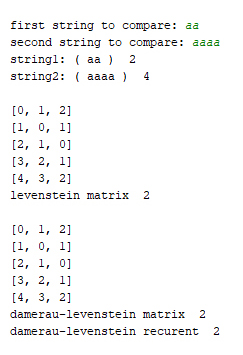
\includegraphics[width=0.6\linewidth]{test6.jpg}
        	\caption{Результат нахождения редакторского расстояния при добавлении символов в первую строку}
        	\label{ris:test1}
        \end{figure}
    
    	\newpage
    	\begin{figure}[h!]
    		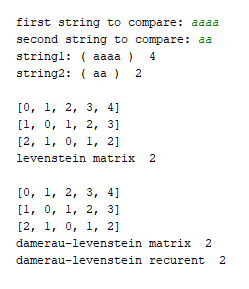
\includegraphics[width=0.6\linewidth]{test5.jpg}
    		\caption{Результат нахождения редакторского расстояния при удалении символов из первой строки}
    		\label{ris:test2}
    	\end{figure}
    
    	\newpage
    	\begin{figure}[h!]
    		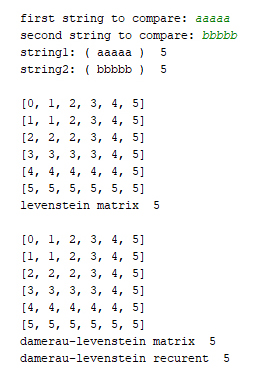
\includegraphics[width=0.6\linewidth]{test4.jpg}
    		\caption{Результат нахождения редакторского расстояния при замене символов первой строки}
    		\label{ris:test3}
    	\end{figure}
    
    	\newpage
    	\begin{figure}[h!]
    		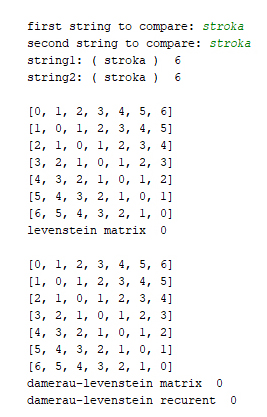
\includegraphics[width=0.6\linewidth]{test3.jpg}
    		\caption{Результат нахождения редакторского расстояния при совпадении символов в первой строке}
    		\label{ris:test4}
    	\end{figure}
    
    	\newpage
    	\begin{figure}[h!]
    		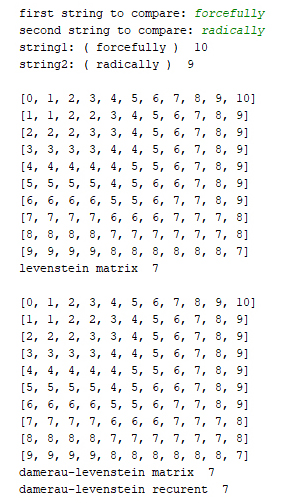
\includegraphics[width=0.6\linewidth]{test2.jpg}
    		\caption{Результат нахождения редакторского расстояния}
    		\label{ris:test5}
    	\end{figure}
    
    	\newpage
    	\begin{figure}[h!]
    		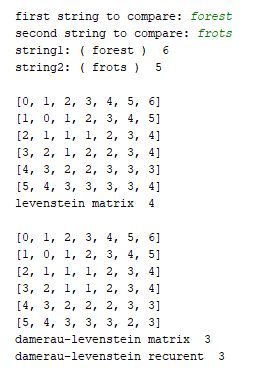
\includegraphics[width=0.6\linewidth]{test1.jpg}
    		\caption{Сравнение нахождения редакторского расстояния Левенштейна и Дамерау-Левенштейна}
    		\label{ris:test6}
    	\end{figure}

		\newpage
        \textbf{4.2. Сравнительный анализ на материале экспериментальных данных}
        \begin{flushleft}
        	В ходе эксперимента были полученны следующие данные:\\
        	\begin{figure}[h!]
        		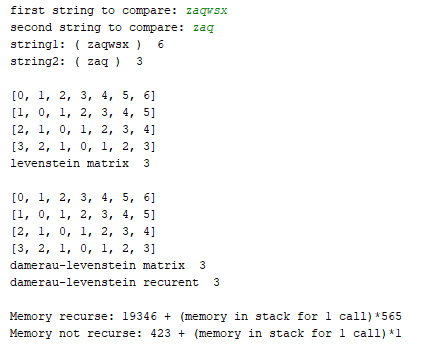
\includegraphics[width=1\linewidth]{test7.jpg}
        		\caption{Использование памяти разными реализациями алгоритма. Пример 1}
        		\label{ris:test7}
        	\end{figure}

			\newpage
			\begin{figure}[h!]
				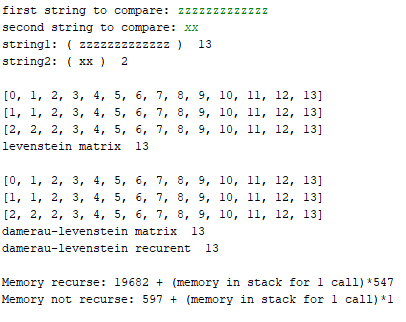
\includegraphics[width=1\linewidth]{test10.jpg}
				\caption{Использование памяти разными реализациями алгоритма. Пример 2}
				\label{ris:test8}
			\end{figure}
		
			\newpage
			\begin{figure}[h!]
				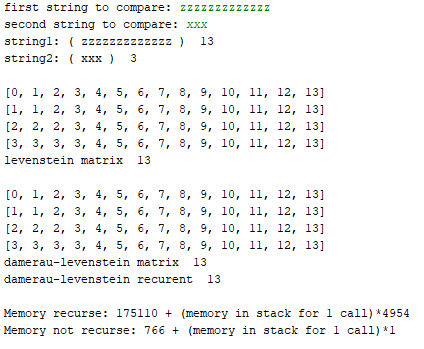
\includegraphics[width=1\linewidth]{test9.jpg}
				\caption{Использование памяти разными реализациями алгоритма. Пример 3}
				\label{ris:test9}
			\end{figure}
		
			\newpage
			\begin{figure}[h!]
				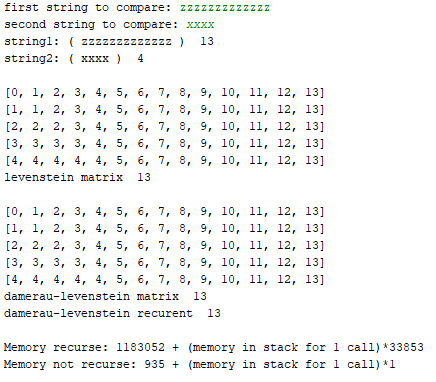
\includegraphics[width=1\linewidth]{test8.jpg}
				\caption{Использование памяти разными реализациями алгоритма. Пример 4}
				\label{ris:test10}
			\end{figure}
 
 			\newpage
 				\begin{tikzpicture}
 				\begin{axis}[
 				ylabel = Время\, секунды, xlabel = Длина\, символы,
 				width = 500, height = 600
 				]
 				\addplot coordinates {
 					(2,0.0000469) (3,0.0000517) (4,0.0001219) (5,0.0001213) (6,0.0000956) (7,0.0001706) (8,0.0001937) (9,0.0002775) (10,0.0003219)
 				};
 				\addlegendentry{Матричный алгоритм Дамерау-Левенштейна}
 				\addplot coordinates {
 					(2,0.0000313) (3,0.0000469) (4,0.0000938) (5,0.0001094) (6,0.0000781) 	(7,0.0001563) (8,0.0001719) (9,0.0002344) (10,0.0002969)
 				};
 				\addlegendentry{Матричный алгоритм Левенштейна}
 				\end{axis}
 				\end{tikzpicture}
 
 				\begin{tikzpicture}
 				\begin{axis}[
 				ylabel = Время\, секунды, xlabel = Длина\, символы,
 				width = 500, height = 600
 				]
 				\addplot coordinates {
 					(2,0.0000469) (3,0.0002344) (4,0.0011719) (5,0.0035313) (6,0.0192656) (7,0.1056406) (8,0.6040937) (9,3.4721875) (10,16.6491719)
 				};
 				\addlegendentry{Рекурсивный алгоритм Дамерау-Левенштейна}
 				\addplot coordinates {
 					(2,0.0000313) (3,0.0000469) (4,0.0000938) (5,0.0001094) (6,0.0000781) 	(7,0.0001563) (8,0.0001719) (9,0.0002344) (10,0.0002969)
 				};
 				\addlegendentry{Матричный алгоритм Дамерау-Левенштейна}
 				\end{axis}
 				\end{tikzpicture}
        \end{flushleft}
        
        \textbf{4.3. Вывод из экспериментов}
        \begin{flushleft}
        	Рекурсивный алгоритм проще для реализации, но на длинных входных строках (в рамках лабораторной для этого алгоритма строки уже длиной 9 являлись длительно обрабатываемыми) оказывается неэффективным как по памяти, так и времени выполнения. Матричная реализация данного алгоритма в аналогичных условиях потребляет в разы меньше памяти и работает быстрее.
        \end{flushleft}
    \end{center}

    \newpage

    \begin{center}
        \textbf{Заключение}
        \label{sec:conclusion_part}
    \end{center}
        
        	В результате выполнения данной работы рассмотренны и изучены понятия расстояния Левенштейна и расстояния Дамерау-Левенштейна. Реализован матричный вариант алгоритма нахождения расстояния Левенштейна. Реализовано два варианта алгоритма нахождения расстояния Дамерау-Левенштейна (в рекурсивной и матричной формах). Сравнены их временные характеристики как следствие проведённых экспериментов. Были сделаны выводы об эффективности по времени рекурсивного и нерекурсивного вариантов алгоритмов.
       

\end{document}
